\chapter[INTERSCITY]{INTERSCITY}

Com o objetivo de prover uma solução para os problemas presentes no ecossistema
de cidades inteligentes, surge o InterSCity, uma plataforma que foca em
aspectos como interoperabilidade, escalabilidade, extensibilidade, e qualidade,
licenciado sob
MPLv2 \footnote{\url{www.mozilla.org/en-US/MPL/2.0/}}, e construído
utilizando a arquitetura de microserviços -
MSA \footnote{\url{microservices.io/}} \cite{delesposte2017}.

Baseando-se no desenvolvimento colaborativo e na utilização de tecnologias
software livre de ponta, o InterSCity conta atualmente com a ajuda de diversos
colaboradores, e, utilizando metodologias ágeis, mantém sua evolução ao longo
do tempo \cite{delesposte2017}.

Escrito majoritariamente em Ruby on Rails\footnote{\url{rubyonrails.org/}},
a plataforma segue padrões que priorizam extensibilidade e qualidade, e
apresenta uma arquitetura madura e bem planejada. O InterSCity se encontra
hospedado no Gitlab \footnote{\url{gitlab.com/smart-city-software-platform}},
onde cada um de seus microserviços têm um repositório. Outros recursos
importantes como: documentação da arquitetura, um cliente exemplo para
confecção de novos dispositivo IoT para serem usados na plataforma, dentre
outros itens, também podem ser encontrados no repositório.

Durante o detalhamento do InterSCity, os microserviços serão chamados
intermitentemente de \textit{módulos} e \textit{componentes}. % precisa falar isso?

\section{PRINCÍPIOS}

O InterSCity foi desenvolvido utilizando princípios de \textit{design}, e,
assim, busca atender critérios estabelecidos. Os princípios são:

\begin{itemize}
    \item \textbf{Modularidade através de serviços}: O InterSCity se torna mais
modular através da criação de mais microserviços, que buscam ter
responsabilidades atômicas e bem definidas \cite{delesposte2017}.

    \item \textbf{Modelos e Dados Distribuídos}: O InterSCity melhora sua
escalabilidade através da distribuição dos dados e dos modelos. Com essa
prática, cada microserviço pode evoluir separadamente, por contar com seu
próprio banco de dados \cite{delesposte2017}. Contudo, esse princípio apresenta
o ponto negativo de aumentar a complexidade.

    \item \textbf{Evolução Descentralizada}: Por conta do não-acoplamento, é
possível que módulos do InterSCity evoluam e sofram manutenção
independentemente, sem afetar outros microserviços da plataforma
\cite{delesposte2017}.

    \item \textbf{Reuso de Projetos de Código Aberto}: O InterSCity preferencia % uso software livre ou codigo aberto?
projetos robustos já desenvolvidos, ao invés de desenvolver soluções do zero
\cite{delesposte2017}. Contudo, esta escolha é feita com cuidado, e somente
projetos com colaboradores e mantenedores ativos, e com documentação
apropriada, são utilizadas na plataforma \cite{delesposte2017}.

    \item \textbf{Adoção de Padrões Abertos}: O InterSCity adota padrões já
difundidos, para que seja provida maior interoperabilidade entre a plataforma
e outros projetos \cite{delesposte2017}.

    \item \textbf{Assíncrono contra Síncrono}: O InterSCity busca prover
serviços e atividades assíncronas sempre que possível, com a finalidade de
evitar que eventos blocantes ocorram. Isto é atingido principalmente através
do padrão PubSub, e de estratégias baseadas em eventos \cite{delesposte2017}.

    \item \textbf{Serviços sem Estado}: Os microserviços do InterSCity evitam,
sempre que possível, ter um estado específico \cite{delesposte2017}. Com isso,
os microserviços podem responder a qualquer requisição a qualquer momento, ao
contrário do que ocorreria caso tivessem estados específicos, pois só
conseguiriam caso certas transições ocorressem.
\end{itemize}

\section{ARQUITETURA}

O InterSCity apresenta uma arquitetura de microserviços distribuída, e conta
atualmente com os microserviços Resource Adaptor, Resource Viewer,
Resource Catalog, Data Collector, Resource Discovery, e Actuator Controller.
Estes componentes são desacoplados entre si, e cada um tem
responsabilidades específicas e bem definidas. A comunicação entre eles é
feita via RabbitMQ\footnote{\url{www.rabbitmq.com/}}, através
do padrão de projeto PubSub\footnote{\url{xmpp.org/extensions/xep-0060.html}},
ou via requisições REST. O modelo de comunicação via passagem de mensagem é
importante em contextos de concorrência pelo isolamento provido
\cite{armstrong2003}, e é chave na ligação entre os diferentes módulos do
InterSCity.

\begin{figure}
  \centering
    \includegraphics[scale=0.5]{figuras/interscity-flow.png}
  \caption{Ciclo de vida de um recurso IoT no InterSCity.}
  \label{fig:interscity-lifecycle}
\end{figure}

A figura \ref{fig:interscity-lifecycle} ilustra um ciclo de vida típico de um
recurso IoT na plataforma. Inicialmente, o recurso (i) começa um pedido de
registro na plataforma com o Resource Adaptor, que, (ii) gerenciando a conversa
com o módulo Resource Catalog, (iii) informa ao recurso seu UUID, que será
utilizado internamente deste passo em diante. Após, a comunicação entre o
Resource Adaptor e o dispositivo IoT ainda continuará, mas, (iv) os dados terão
como destino o módulo Data Collector, que armazenará as informações. Por fim,
(vi) as informações contidas no Data Collector serão enviadas para o
Resource Viewer, apresentando então os dados do recurso para o usuário final.
% adicionar imagem?
% preciso referenciar?

\section{MICROSERVIÇOS}

\begin{itemize}
    \item \textbf{Resource Adaptor}: é o grande responsável pela comunicação
entre os dispositivos IoT e o InterSCity, e funciona como um recepcionista
durante as requisições, gerenciando o registro e atualização dos
dispositivos IoT, e redirecionando informações importantes dos recursos
registrados para os destinos desejados \cite{delesposte2017}. É escrito em
Ruby on Rails, e, embora converse com os recursos IoT diretamente, comunica-se
com alguns dos microserviços da plataforma via RabbitMQ.

    \item \textbf{Data Collector}: tem como papel o armazenamento e
disponibilização de dados coletados pelos recursos registrados na plataforma
\cite{delesposte2017}. Também escrito em Ruby on Rails, este microserviço fará
contínua comunicação com a camada de processamento que será desenvolvida.
Constantemente publica dados em tópicos do RabbitMQ, que serão consumidos por
outros microserviços, contudo, a comunicação com o Resource Viewer é feita
diretamente, e não por passagem de mensagem. Os recursos armazenados são
expostos via API, disponibilizando também dados históricos.

    \item \textbf{Resource Viewer}: o único microserviço da plataforma escrito em
EmberJS\footnote{\url{www.emberjs.com/}}, e tem o papel de apresentar os dados
armazenados no Data Collector e no Resource Catalog para o usuário final
\cite{delesposte2017}. Após a adição do módulo de processamento, é esperado que
o Resource Viewer passe a apresentar também os dados processados.

    \item \textbf{Resource Catalog}: gerencia o registro e o estado de recursos
IoT na plataforma. Este microserviço, escrito em Ruby on Rails, fornece
identificadores únicos (UUID) para cada recurso que se registra na plataforma
\cite{delesposte2017}. O identificador único será utilizado então nas futuras
comunicações que ocorrerão, tanto via RabbitMQ quanto via requisição REST.

    \item \textbf{Resource Discovery}: responsável por prover uma API para a
descoberta dos recursos IoT disponíveis, com possibilidade de uso de filtros
diversos \cite{delesposte2017}.

    \item \textbf{Actuator Controller}: provê serviços para requisições nos
recursos IoT atuadores registrados na plataforma\cite{delesposte2017}. Estas
requisições são armazenadas, e podem ser recuperadas no futuro para fins
de auditoria \cite{delesposte2017}.

\end{itemize}

\section{PERFORMANCE}

Para mensurar a performance do InterSCity, dois experimentos foram feitos:
um, para avaliar a degradação da performance conforme o número de clientes
enviando dados concorrentemente aumenta; e outra análise, com mudanças na % posso usar ponto e virgula?
infraestrutura, com o objetivo de mensurar o quanto a performance melhorou
com o aumento dos recursos computacionais \cite{delesposte2017}.

\begin{figure}
  \centering
    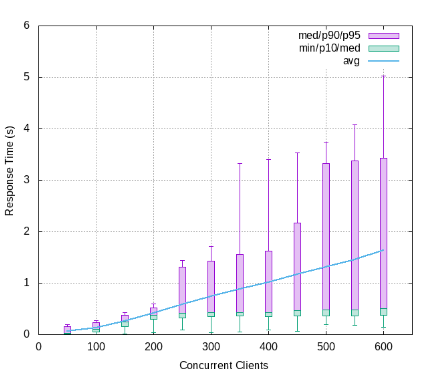
\includegraphics[scale=0.7]{figuras/benchmark1.png}
    \caption{Degradação no tempo de resposta. Fonte: ESPOSTE, 2017.}
  \label{fig:benchmark1}
\end{figure}

No primeiro experimento, clientes ficaram em um laço de repetição enviando
dados por requisições síncronas durante 4 minutos. O experimento foi feito
utilizando 11 diferentes configurações, variando o número de clientes
concorrentes. Com os resultados, que estão apresentados na figura
\ref{fig:benchmark1}, pôde ser percebido que: (i) o microserviço
Resource Adaptor manteve o maior uso dos recursos, sendo considerado o
maior gargalo da plataforma, juntamente com o Data Collector, que também
apresentou uso intensivo da CPU; (ii) para 50 clientes concorrentes, o
tempo de resposta médio foi de 60 milissegundos; (iii) acima de 250 clientes
concorrentes, as requisições passaram a ter latência de 1 segundo
\cite{delesposte2017}.

\begin{figure}
  \centering
    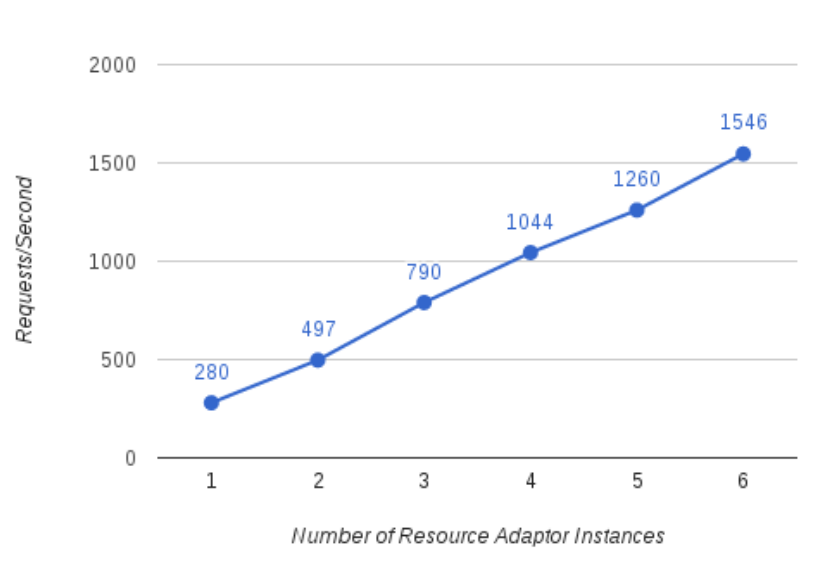
\includegraphics[scale=0.4]{figuras/benchmark2.png}
    \caption{Número de requisições por segundo com aumento de recursos. Fonte: ESPOSTE, 2017.}
  \label{fig:benchmark2}
\end{figure}

No segundo experimento, um cenário de 500 clientes concorrentes foi utilizado, 
durante 6 ciclos de 4 minutos, e com diferentes configurações de
\textit{hardware}, melhorando os recursos computacionais. Foi utilizado
balanceamento de carga igualitário (\textit{round-robin}) nos serviços
que foram identificados como os gargalos da plataforma - isto foi possível
graças aos princípios seguidos, mencionados anteriormente. Os resultados,
que estão apresentados na figura \ref{fig:benchmark2}, permitem concluir que:
(i) só é necessário a melhora de alguns microserviços para melhor desempenho
da plataforma, até certo ponto; (ii) a plataforma consegue escalar linearmente
com a adição de recursos, o que mostra o quão escalável é o InterSCity. Além
disso, foi observado que, por conta do alto número de clientes, o RabbitMQ
passou a consumir grandes recursos, o que o trás como outro possível gargalo,
caso tenha disponível pouco recurso computacional \cite{delesposte2017}.

\section{GERÊNCIA DE CONFIGURAÇÃO}

Outro aspecto que recebe atenção no desenvolvimento do InterSCity é a gerência
de configuração, que, atualmente, utiliza tecnologias de ponta, que reduzem
trabalho desnecessário, ao passo em que promovem isolamento entre a plataforma
e o ambiente hospedeiro. A gerência de configuração do InterSCity é guiada por
\textit{containers} do Docker\footnote{\url{https://www.docker.com/}}, e cada
microserviço e serviço externo (como o RabbitMQ) é executado em
\textit{containers} separados; e pelo uso do
Git\footnote{\url{https://git-scm.com/}}. Assim, a configuração de um ambiente
para execução do InterSCity tem como pré-requisitos a instalação do Docker, do
Docker Compose e do Git.

Um repositório principal, chamado
\textit{dev-env}\footnote{\url{https://gitlab.com/smart-city-software-platform/dev-env}},
funciona como \textit{projeto mestre}, e os microserviços da plataforma são
submódulos pertencentes a este. Desta forma, os estados do projeto mestre são
ligados aos estados dos microserviços, garantindo compatibilidade. Por exemplo:
o cenário de um microserviço precisar utilizar uma versão recente de outro
microserviço, mas este estar numa versão mais antiga, não acontece sem que seja
desejado.

Os passos para configuração do InterSCity são os seguintes:

% configura o lstlisting:
\lstset{
    tabsize=4,
    rulecolor=,
    language=bash,
    basicstyle=\scriptsize,
    columns=fixed,
    showstringspaces=false,
    breaklines=true
}
\begin{enumerate}
    \item Clonar o repositório principal, iniciar submódulos e atualizar submódulos:
        \begin{lstlisting}[basicstyle=\tiny,]
        $ git clone https://gitlab.com/smart-city-software-platform/dev-env.git
        $ git submodule init
        $ git submodule update
        \end{lstlisting}

    \item Executar o \textit{setup} do arquivo de configuração do projeto:
        \begin{lstlisting}
        $ ./project setup
        \end{lstlisting}

    \item Executar a rotina \textit{start} no arquivo de configuração:
        \begin{lstlisting}
        $ ./project start
        \end{lstlisting}
\end{enumerate}

Os módulos do InterSCity passarão então a rodar nas diferentes portas
desejadas. Os estados dos serviços podem ser conferidos através do comando
\begin{lstlisting}
$ docker ps
\end{lstlisting}

% necessário? abaixo
A partir dos pontos levantados, é possível analisar o nível de maturidade do
InterSCity. Mesmo sendo distribuído (pela arquitetura), escalável (provado
pelos experimentos), e bem configurado (pela gerência de configuração), o
projeto ainda não faz uso de tecnologias Big Data. No próximo capítulo serão
apresentadas duas arquiteturas Big Data bem difundidas, e, em seguida, será
levantada a proposta de arquitetura para a camada de processamento de dados.
